\documentclass[12pt]{article}
\usepackage{text_style}
\title{Forward and inverse problems in causal discovery}
\author{IA pour la Science}
\date{23 April 2026}
\begin{document}
\maketitle
%\begin{abstract}
%This document explains the scheme of causal structure selection and generation
%\end{abstract}

\section{Functional diagram of the model forecasting}
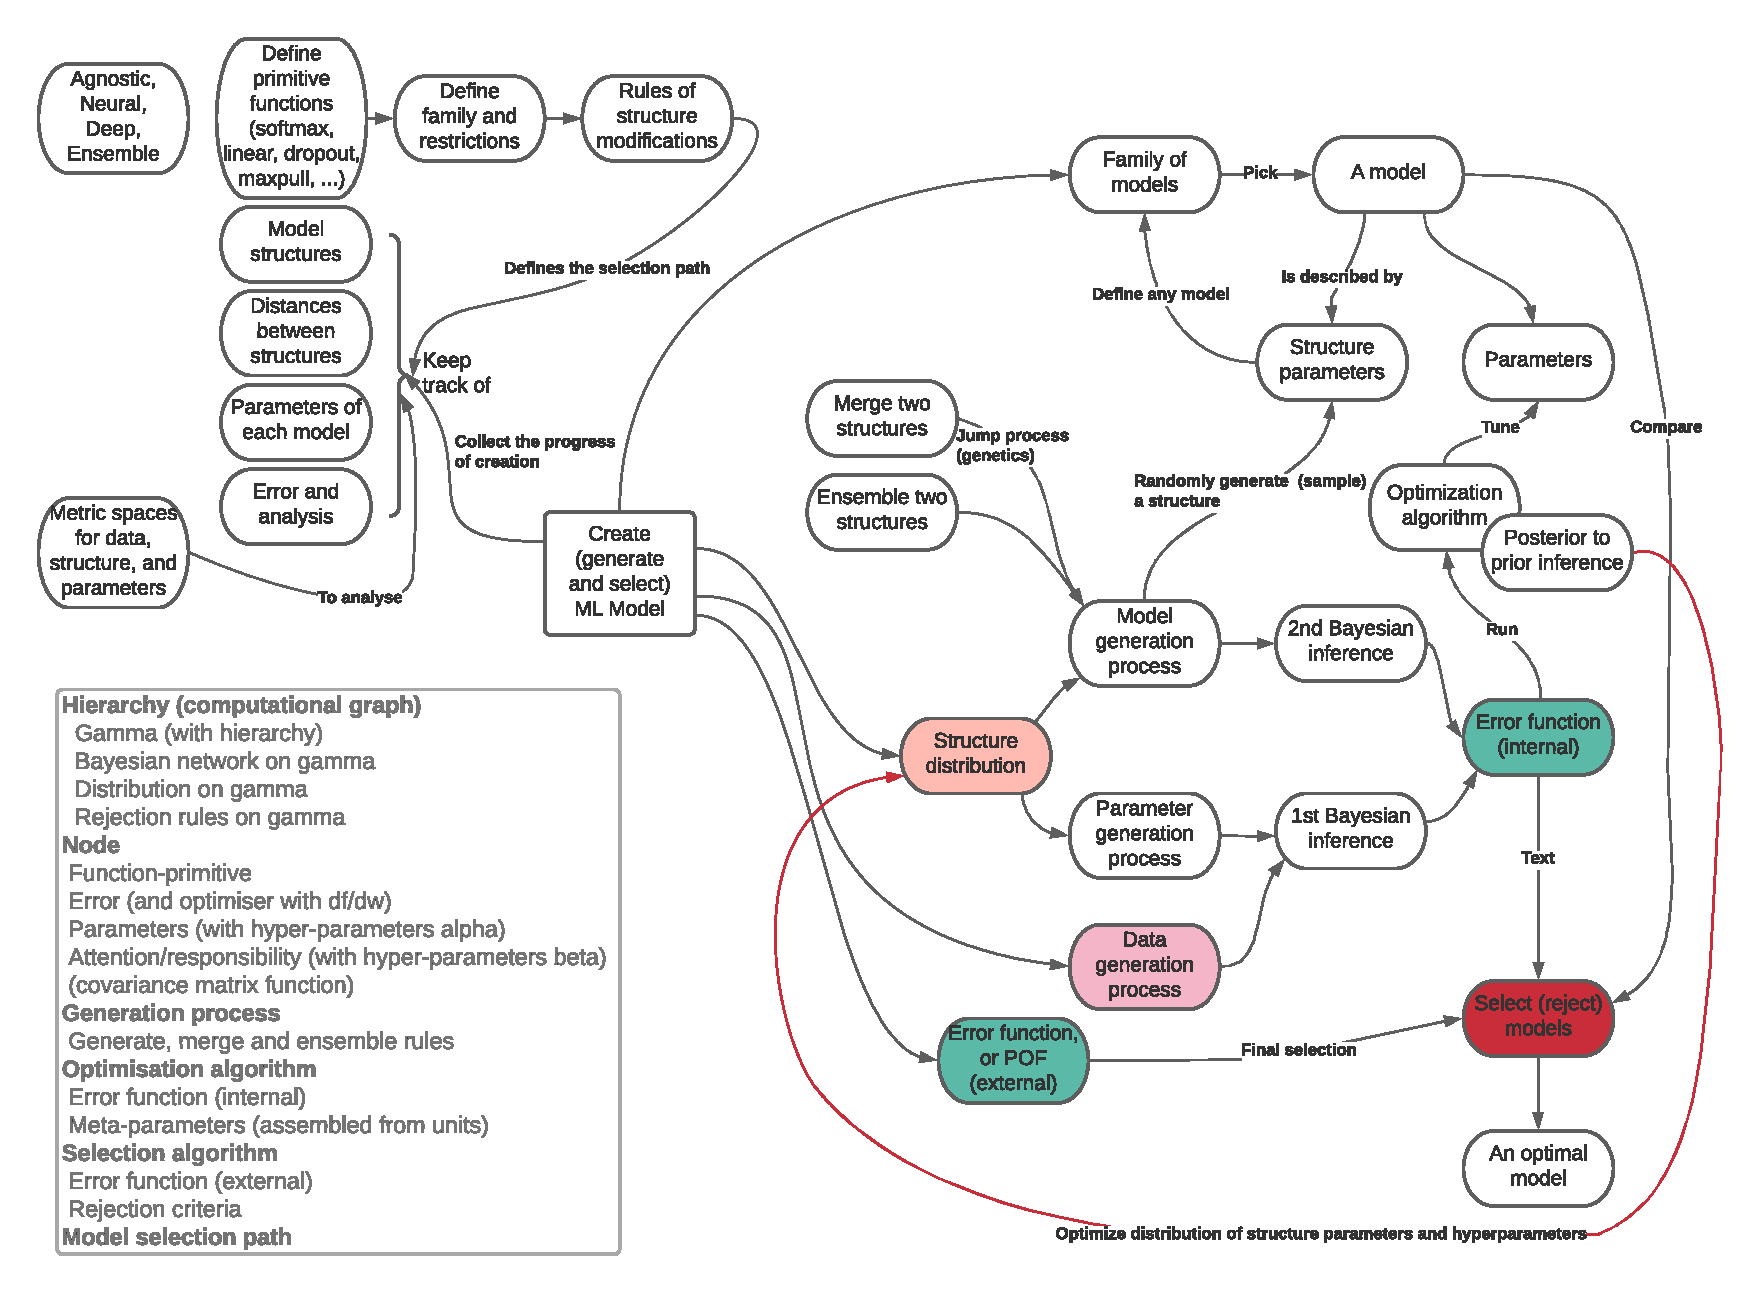
\includegraphics[width=\textwidth]{intro_structure_learning_map.pdf}

\section{Generall problem statement in multimodeling}
\includegraphics[width=\textwidth]{tmp/fig_multi_mod_1}

\section{When do we need a multimodel}
\includegraphics[width=\textwidth]{tmp/fig_multi_mod_2}

\section{Model comparison hypotheses}
\includegraphics[width=\textwidth]{tmp/fig_multi_mod_3}

\section{Proposed statement of the model comparison}
\includegraphics[width=\textwidth]{tmp/fig_multi_mod_4}

\section{Explicit form of $s(g_1,g_2)$ for a pair of normal distributions}
\includegraphics[width=\textwidth]{tmp/fig_multi_mod_5}

\section{Mixture of experts as a multimodel}
\includegraphics[width=\textwidth]{tmp/fig_multi_mod_6}

\section{Similarity of models in a multimodel}
\includegraphics[width=\textwidth]{tmp/fig_multi_mod_7}

\section{Model comparison issues}
\includegraphics[width=\textwidth]{tmp/fig_multi_mod_8}

\section{Requirements to the similarity function}
\includegraphics[width=\textwidth]{tmp/fig_multi_mod_9}
\end{document}